%!TEX root = ../slide.tex

\begin{frame}{Why I started a PhD ?}{3 main reasons}
	\begin{itemize}
		\item Research methodology lecture.
		\item Bac+5 in networking ? not really !
		\item Being paid to study and to develop yourself !
	\end{itemize}
\end{frame}

% \subsection{IoT Devices}
\begin{frame}{IoT devices}{IoT devices are useless without a good communication capability}
	\centering
	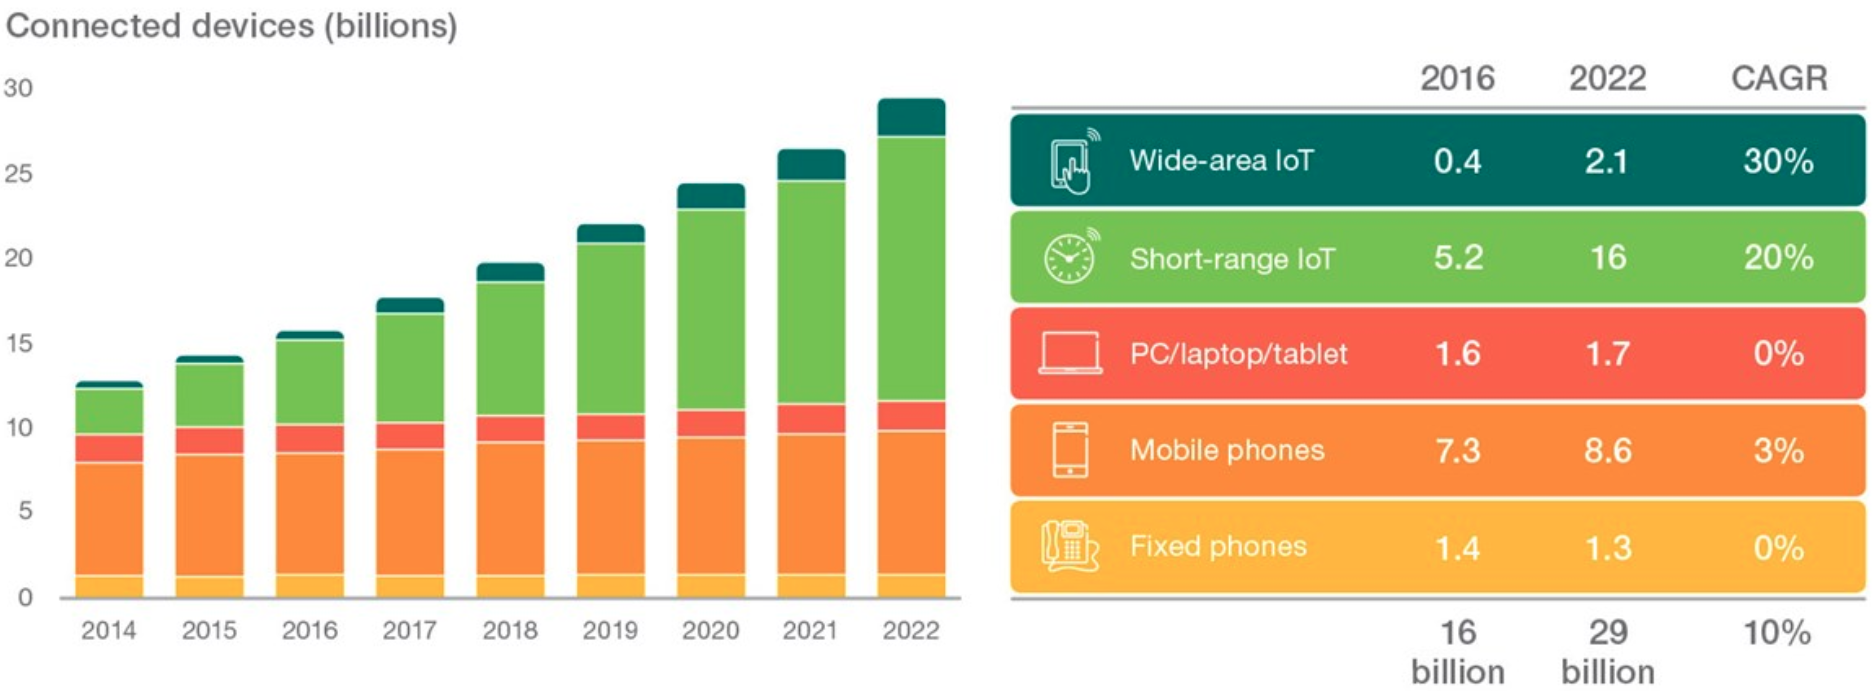
\includegraphics[width=.9\columnwidth]{devices1}
	\Figure{!htb}{1}{devices}{IoT devices \cite{perera_mosden_2013}}
	% \Figure{!htb}{.7}{devices.jpg}{IoT devices \cite{perera_mosden_2013}}
\end{frame}

% \subsection{IoT Applications}
\begin{frame}{IoT applications requirements}{Each application has its own communication requirements}
	\Columns{0.6}{0.4}{
		\begin{table}[h!]
		\scriptsize
			\begin{tabulary}{\textwidth}{L|C|C|C|C|C}
			Challenges/Applications & Grids 	  & EHealth   & Transport 	  & Cities 		 & \textbf{Building}	\\\hline
			Resources constraints   & \ko         & \ok		  & \ko           & \mm          & \ko            		\\\hline
			Mobility                & \ko         & \mm    	  & \ok           & \ok          & \ko            		\\\hline
			\textbf{Heterogeneity}  & \mm 	      & \mm    	  & \mm           & \ok          & \ko            		\\\hline
			Scalability             & \ok 		  & \mm       & \ok           & \ok          & \mm           	 	\\\hline
			QoS constraints         & \mm 	      & \mm       & \ok           & \ok          & \ok              	\\\hline
			Data management         & \mm 	      & \ko       & \ok           & \ok          & \mm              	\\\hline
			Lack of Standardization & \mm     	  & \mm 	  & \mm 	      & \mm          & \ok              	\\\hline
			Amount of attacks       & \ko         & \ko       & \ok 		  & \ok          & \ok              	\\\hline
			Safety                  & \mm 	      & \ok 	  & \ok		      & \mm          & \ok               	\\\hline
			\end{tabulary}
		\caption{\label{tab:iot_challenges} Main IoT challenges \cite{kouicem_internet_2018} \cite{venkatesan_design_2017}}
		\end{table}
	}{
		\Figure{!htb}{1}{application}{IoT Applications}
	}
\end{frame}

% Current bad state, statistics with the problem
% \subsection{Context}
\begin{frame}{IoT platforms}{IoT platforms is a chain of communication process}
	\Figure{!htb}{.8}{context}{IoT platform}
	\Figure{!htb}{.9}{iotChallenges}{IoT challenges}
\end{frame}


\begin{frame}{IoT applications requirements}{Context} 
\begin{table}[h!]
\scriptsize
	\begin{tabulary}{\columnwidth}{L|C|C|L}
	\textbf{Use Case}                      & \textbf{Packet rate} 	& \textbf{Min success rate} & \textbf{Payload Size}						\\
	\				                       & \textbf{[pkt/day]}		& \textbf{[Ps,min]} 		& \textbf{[Byte]}							\\\hline
	\textbf{Wearables}                     & 10                     &        90                 & \multirow{5}{*}{10-20} 	\\
	\textbf{Smoke Detectors}               & 2                      &        90                 &        	 							\\
	\textbf{Smart Grid}                    & 10                     &        90                 &         								\\
	\textbf{White Goods}                   & 3                      &        90                 &         \\
	\textbf{Waste Management}              & 24                     &        90                 &         \\\hline
	\textbf{VIP/Pet Tracking}              & 48                     &        90                 & \multirow{9}{*}{50}        \\
	\textbf{Smart Bicycle}                 & 192                    &        90                 &         \\
	\textbf{Animal Tracking}               & 100                    &        90                 &         \\
	\textbf{Environmental Monitoring}      & 5                      &        90                 &         \\
	\textbf{Asset Tracking}                & 100                    &        90                 &         \\
	\textbf{Smart Parking}                 & 60                     &        90                 &         \\
	\textbf{Alarms/Actuators}              & 5                      &        90                 &         \\
	\textbf{Home Automation}               & 5                      &        90                 &         \\
	\textbf{Machinery Control}             & 100                    &        90                 &         \\\hline
	\textbf{Water/Gas Metering}            & 8                      &        90                 & \multirow{9}{*}{100-200}        \\
	\textbf{Environmental Data Collection} & 24                     &        90                 &         \\
	\textbf{Medical Assisted Living}       & 8                      &        90                 &         \\
	\textbf{Micro-generation}              & 2                      &        90                 &         \\
	\textbf{Safety Monitoring}             & 2                      &        90                 &         \\
	\textbf{Propane Tank Monitoring}       & 2                      &        90                 &         \\
	\textbf{Stationary Monitoring}         & 4                      &        90                 &         \\
	\textbf{Urban Lighting}                & 5                      &        90                 &         \\
	\textbf{Vending Machines Payment}      & 100                    &        90                 &         \\\hline
	\textbf{Vending Machines General}      & 1                      &        90                 & 1K        \\
	\end{tabulary}
\caption{\label{tab:zzes}Application requirements for the use cases of interest \cite{feltrin_lorawan_2018} \cite{venkatesan_design_2017}.}
\end{table}
\end{frame}

% \subsection{IoT Communications}
\begin{frame}{IoT wireless communication}{Wireless communication performance need to be evaluated to match applications requirements}
	\Columns{0.4}{0.6}{
		\Figure{!htb}{1}{speaking}{Human voice}
	}{
		\Figure{!htb}{1}{snr}{SNR \& RSSI}
		\Figure{!htb}{1}{ToA}{Time on air}
	}
\end{frame}

\begin{frame}{Problem statement}{Introduction \footcite{dimartino_internet_2018} ?}
\Columns{.5}{.5}{
	\begin{itemize}
	\item Parameters
		\begin{itemize}
		\item \ac{BW}
		\item \ac{SF}
		\item \ac{CR}
		\item \ac{Tx}
		\end{itemize}
	\end{itemize}
}{
	\begin{itemize}
	\item Metrics
		\begin{itemize}
		\item \ac{RS}
		\item \ac{SNR}
		\item \ac{DR}
		\item \ac{AT}
		\item \ac{PktL}
		\end{itemize}
	\end{itemize}
}

\medskip
\begin{table}[h!]
% \scriptsize
	\begin{tabular}{l|m{1mm}l|l|l}
	\textbf{Setting}& \multicolumn{2}{l|}{\textbf{Values}} 				    & \textbf{Rewards}		   & \textbf{Costs} 					    \\\hline
	\ac{BW}         & $7.8 $ 	& \ding{224} $500 kHz$  								& \ac{DR}          		   & \ac{RS}, \blue{Range} 			  \\\hline
	\ac{SF}         & $2^{6}$ 	& \ding{224} $2^{12}$ 									& \ac{RS}, \blue{Range}    & \ac{DR}, \ac{SNR}, \ac{PktL}, \ac{Tx}    \\\hline
	\ac{CR}         & $4/5$ 	& \ding{224} $4/8$    								  	& Resilience 			   &  \ac{PktL}, \ac{Tx}, \ac{AT} 				\\\hline
	$P_{tx}$        & $-4$ 		& \ding{224} $20 dBm$    								& \ac{SNR} 				   & \ac{Tx}  								\\\hline
	\end{tabular}
\caption{\label{tab:} \footcite{cattani_experimental_2017}}
\end{table}

\end{frame}


\begin{frame}{IoT wireless communication}{Exp: LPWAN in a new technology that satisfy IoT applications requirements}
	\Columns{0.6}{0.4}{
		\Figure{!htb}{1}{LPWAN}{Wireless communication diversity}
	}{
		\Figure{!htb}{1}{lora_stack}{LoRa and LoraWan stack}
	}
\end{frame}


% Why -> problem, This is due to the lack of
% \subsection*{Problematic}
\begin{frame}{Problematic}{One size fits all problem: 1) Many configurations, 2) Diversity of service requirements}
	\Figure{!htb}{.6}{slicing}{Key barriers in adopting IoT in the industry \cite{sciancalepore_storns_2019}}

	% \bey{How to adapt the network to applications ?}
	\stamp{blue}{30}{6.2, 5}{How to adapt network configurations to applications ?}{90}

\end{frame}

\begin{frame}{Problematic}{Where is the problem ?}
		\Itemize{
			\item Some network configuration are static and not adptive to the application
			\Itemize{
				\item Decision and optimisation problem..
				\item Various network acces
				\item Various configuration of each network acces
				\item Lake of selection tools
			}
			\item Users have to select the network and the application
			\Itemize{
				\item How to select the \textbf{best} network.
				\item How to select the network required by the application.
			}
		}
\end{frame}

% Future good state:  statistics without the problem}
%Who and what could we win if we resolve this probleme, why we didn't let it like it is
% \subsection*{Motivation}
\begin{frame}{End-to-end Network slicing}{Exp: 4G/5G, Content provider (GAFA) want to be directly connected to users devices}
	\Columns{0.5}{0.5}{
		\Figure{!htb}{1}{slicing4}{Network slicing \cite{sciancalepore_storns_2019}}
	}{
		\FigureH{!htb}{1}{4G_slicing}{4G without network slicing}{5G_slicing}{5G with network slicing}{slicing3}{Network slicing concept \cite{sama_servicebased_2016}}
	}
\end{frame}

\begin{frame}{Conclusion}{In the future, network administration function will disappear and will be replaced by a slice orchestrator}
	% \tikz{\draw[red,thick,dashed] (2,2) circle (3cm);}
	% \tikz{\draw[step=1cm,gray,very thin] (-1.9,-1.9) grid (5.9,5.9);}
	\Figure{!htb}{.7}{slicing2}{Slice orchestrator \cite{ksentini_toward_2017}}
	\bey{blue}{0}{6, 4}{\Huge Thank you !}
\end{frame}


\begin{frame}{Contribution}{Contributions}
	\begin{itemize}
		\item \textbf{3 Applications}
		\begin{itemize}
			\item Voice, Images and Text transmission.
		\end{itemize}
	\end{itemize}

	\begin{itemize}
		\item \textbf{3 Environment conditions}
		\begin{itemize}
			\item Rural/Urban
			\item Static/Mobile
			\item Temperature
		\end{itemize}
	\end{itemize}

	\begin{itemize}
		\item \textbf{6 Scenarios}
		\begin{itemize}
			\item Application protocol (MQTT, COAP, XMPP)
			\item Network protocol (Start, Mesh)
			\item MAC protocol (LoraWan, Sigfox, ...)
		\end{itemize}

		\item \textbf{6 algorithms}
		\begin{itemize}
			\item ..
			\item ..
			\item ..
		\end{itemize}

		\item \textbf{Inputs:}
		\begin{itemize}
			\item QoS metrics:
			\Itemize{
				\item User metrics: Cost
				\item Network metrics: Receiver sensitivity, SNR, DR, Air time, Payload length.
			}
			\item MAC configuration (SF, CR, BW, Tx)
		\end{itemize}

		\item \textbf{Outputs:}
		\begin{itemize}
			\item ($SF_{i}, CR_{j}, BW_{k}, Tx_{l}$)
		\end{itemize}
	\end{itemize}
\end{frame}

\begin{frame}{Contribution}{Contributions}
	\Figure{h}{.75}{infocom}{jh}
\end{frame}

% specifique, mesurables, atteignable, réalistic, time ?
% Reduce latency ...
% How can we validate 
% \subsection*{Goal}


